\begin{figure}[htbp]
\centering\footnotesize
\begin{minipage}[t]{0.42\linewidth}
\setlength{\zoomw}{0.465\linewidth}%
\textbf{1. What the agent observed}\par\vspace{3pt}
\begin{tabular}{@{}c@{\hspace{0.05\linewidth}}c@{}}
\begin{markedboard}[\zoomw]{lessons-game-over-a.png}
\draw[black,line width=0.7pt] (0,0) rectangle (0.25,0.0625);
\end{markedboard} &
\begin{markedboard}[\zoomw]{lessons-game-over-b.png}
\draw[black,line width=0.7pt] (0,0) rectangle (0.25,0.0625);
\end{markedboard}\\[1pt]
Before action 357 & After it: game over\\[5pt]
% the boxed corner of each board, four times larger: 16 cells wide, 4 cells high
\begin{tikzpicture}
\begin{scope}\clip (0,0) rectangle (\zoomw,0.25\zoomw);
\node[anchor=south west,inner sep=0pt] at (0,0) {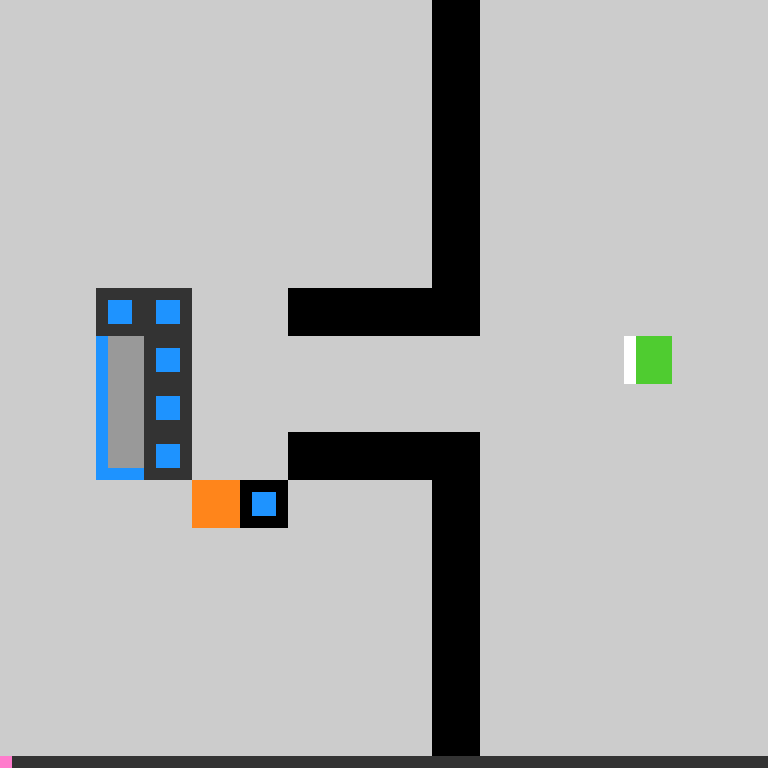
\includegraphics[width=4\zoomw]{figures/runs/lessons-game-over-a.png}};\end{scope}
\draw[black,line width=0.7pt] (0,0) rectangle (\zoomw,0.25\zoomw);
\node[font=\scriptsize,anchor=west,inner sep=1pt] (lab) at (0.2\zoomw,0.16\zoomw) {last pink cell};
\draw[-{Stealth[length=1.6mm]},line width=0.6pt] (lab.west) -- (0.045\zoomw,0.075\zoomw);
\end{tikzpicture} &
\begin{tikzpicture}
\begin{scope}\clip (0,0) rectangle (\zoomw,0.25\zoomw);
\node[anchor=south west,inner sep=0pt] at (0,0) {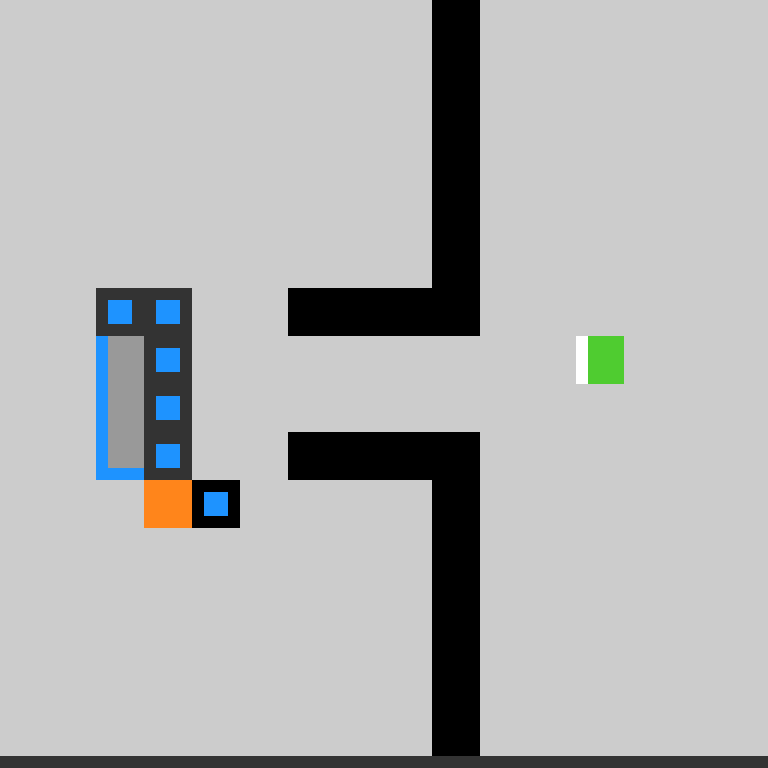
\includegraphics[width=4\zoomw]{figures/runs/lessons-game-over-b.png}};\end{scope}
\draw[black,line width=0.7pt] (0,0) rectangle (\zoomw,0.25\zoomw);
\node[font=\scriptsize,anchor=west,inner sep=1pt] at (0.2\zoomw,0.16\zoomw) {bar empty};
\end{tikzpicture}\\[1pt]
\multicolumn{2}{@{}c@{}}{The boxed corner, four times larger}
\end{tabular}
\end{minipage}\hfill
\begin{minipage}[t]{0.555\linewidth}
\textbf{2. What it stored}, in its reply for action 359\par\vspace{2pt}
\begin{tabularx}{\linewidth}{@{}lY@{}}\toprule
Rule & ``The bar on row 63 is an action budget. Its 7 cells turn to 4 about one every two actions, and the game is over when the last 7 is gone, whatever else is happening on the board.''\\
Applies when & ``Count the 7 cells left on the bottom row and multiply by about 2. If the moves still needed to cover every target tile come to more than that, the attempt will fail. Plan the shortest delivery route from the start and avoid wasted moves.''\\\bottomrule
\end{tabularx}\par\vspace{7pt}
\textbf{3. What the next request showed}, the one for action 360\par\vspace{2pt}
\begin{tabularx}{\linewidth}{@{}lY@{}}\toprule
In the request & The rule and its applies-when clause above, listed under \texttt{game\_over\_lessons} and tagged \texttt{after t357, level 5}\\
The model's check & ``Game-over lesson (budget): 63 of the 64 bottom cells are still 7, so this action will not end the game, and grabbing is needed for the shortest delivery.''\\\bottomrule
\end{tabularx}
\end{minipage}
\caption{\textbf{One game over, the lesson the model wrote from it, and the lesson's return in the next request.} In the layered run of \texttt{wa30}, level 5, action 357 emptied the bar along the bottom row, and the game ended. The controller reset the level, and the model then wrote the lesson in step 2. The harness stored the lesson without checking it and included it in every later request in that game. Step 3 shows the next request and the model's check of its proposed action against the lesson. In the model's text, 7 is the color code of the pink cells and 4 of the dark ones. The model received boards as text; this figure and Figures~\ref{fig:object-ledger} and~\ref{fig:level-brief} draw them in color \citep{dai2026runfigures}. The check in step 3 comes from the run's saved log; the repository records it word for word.}\label{fig:lesson-game-over}
\end{figure}
